\chapter{The multiphysics architecture}\label{chap:multiphysics}
\section{Shared context and evolving state}
\code{DefectiveCrystalBase} constructs the simulation context: parameters and paths, shared mesh ownership, periodic translations, shared polycrystal ownership, optional finite elements, and the base contexts of enabled physics. It also serves microstructure generation. \code{DefectiveCrystal} creates the selected evolving microstructures and advances the simulation.

\code{MicrostructureBase} is the interface each physics implements. \code{MicrostructureContainer} is both a collection of these objects and an implementation of the same interface. Thus the container can forward lifecycle operations and expose aggregate fields without requiring callers to know the concrete type of every physics.
\begin{figure}[htbp]
\centering
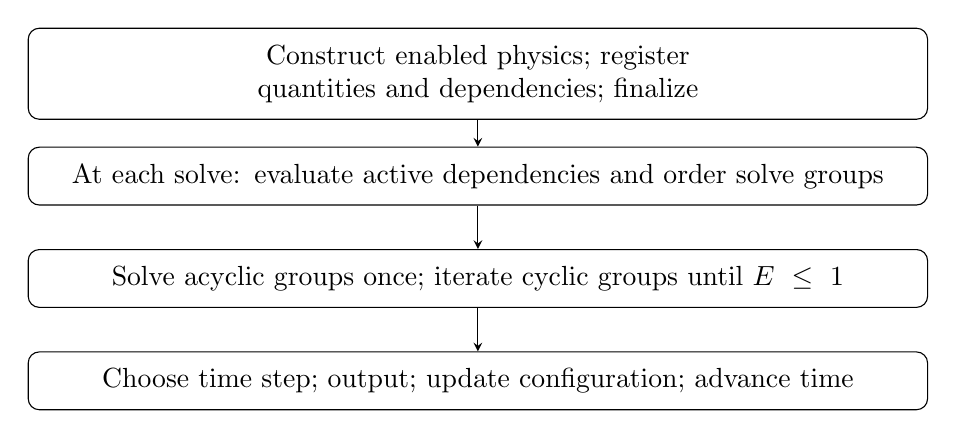
\begin{tikzpicture}[every node/.style={draw,rounded corners,align=center,text width=11cm,inner sep=6pt},>=stealth]
\node (registration) at (0,0) {Construct enabled physics; register quantities and dependencies; finalize};
\node (groups) at (0,-1.3) {At each solve: evaluate active dependencies and order solve groups};
\node (solve) at (0,-2.6) {Solve acyclic groups once; iterate cyclic groups until $E\leq1$};
\node (advance) at (0,-3.9) {Choose time step; output; update configuration; advance time};
\draw[->] (registration) -- (groups);
\draw[->] (groups) -- (solve);
\draw[->] (solve) -- (advance);
\end{tikzpicture}
\caption{Dependency-based multiphysics solution. Geometry and time remain fixed during the solve groups.}
\end{figure}
\sourcefile{include/DefectiveCrystal/DefectiveCrystalBase.h}
\sourcefile{include/DefectiveCrystal/MicrostructureBase.h}
\sourcefile{src/DefectiveCrystal/MicrostructureContainer.cpp}

\section{Lifecycle and common field queries}
The interface includes initialization from a configuration, \code{solve()}, \code{getDt()}, \code{output()} and \code{updateConfiguration()}. It also exposes stress, displacement, inelastic displacement rate, mobile concentrations, immobile clusters, and volume-average quantities. A physics contributes the quantities it represents and returns the appropriate zero contribution for others.

The container sums returned fields. For example,
\begin{equation}
\bm\sigma(\bm x)=\sum_\alpha\bm\sigma^{(\alpha)}(\bm x),\qquad
\langle\bm\beta^P\rangle=\sum_\alpha\langle\bm\beta^{P,(\alpha)}\rangle.
\end{equation}
This additive interface makes coupling accessible, but the module must still define which part of the field it owns. In particular, an elastic correction must not double-count a dislocation's analytical stress. The optional node, element and simplex arguments of field queries provide geometric context and can avoid redundant searches.

\section{Solved quantities and solve groups}\label{sec:solvedQuantities}
The solution order is determined by dependencies between quantities, rather than by the order of physics names in the input. \code{MicrostructureContainer} owns a \code{SolvedQuantityRegistry} and its ordered \code{SolvedQuantityGroup} objects. After constructing all enabled physics, \code{DefectiveCrystal} explicitly calls \code{finalizeSolvedQuantities()}. Each physics registers its operations through \code{registerSolvedQuantities()}.

A \code{SolvedQuantityContribution} describes one update operation: its provider and name, the quantities it publishes, the quantities it needs, and its update callback. One operation can publish several quantities. For example, the DD velocity operation also publishes the dislocation contribution to mobile concentration. Dependencies can select all other providers of a quantity or a particular named provider. A required dependency without a provider is an error; optional dependencies accommodate disabled physics.

At the start of each solve, the registry evaluates conditional dependencies and constructs the directed dependency graph. It finds strongly connected components and orders them so that prerequisites are available first. An acyclic operation is solved once. Operations connected by a dependency cycle form a coupled group and are iterated to convergence. The graph can change between glide and climb steps: concentration feedback is active during climb, but not during glide.

Within a coupled group, operations execute sequentially in a deterministic order, using the latest available results from earlier operations in the same iteration. This is a block fixed-point iteration of Gauss--Seidel type, not a monolithic Newton solve. A group must converge before downstream groups execute.
\sourcefile{include/DefectiveCrystal/SolvedQuantityRegistry.h}
\sourcefile{src/DefectiveCrystal/SolvedQuantityRegistry.cpp}

\subsection{Example: coupled dislocation climb and diffusion}
For a DD/CD/ED climb calculation, a typical sequence is:
\begin{lstlisting}
Solve sequence (5 groups):
  Group 1 [solve once]
    DislocationDynamics:Stress
  Group 2 [solve once]
    ElasticDeformation:Stress
  Group 3 [iterate to convergence]
    ClusterDynamics:MobileConcentration
    DislocationDynamics:Velocity
  Group 4 [solve once]
    ClusterDynamics:ImmobileRates
  Group 5 [solve once]
    ElasticDeformation:DisplacementRate
\end{lstlisting}
The DD stress operation makes the geometry-dependent analytical field available; it does not solve a separate stress system. ED computes the elastic correction before the concentration--velocity iteration. CD concentrations affect climb velocities, while climb velocities affect the dislocation concentration contribution used in CD boundary conditions. These two operations therefore form a cycle. Immobile rates and inelastic displacement rates are evaluated after that cycle converges.

This is an example, not a hard-coded five-stage schedule. The enabled physics and active dependencies determine the groups. DDomp prints the sequence on the first solve and again if its structure changes, rather than repeating an unchanged sequence at every time step.

\section{Convergence control}\label{sec:coupledTolerance}
Each operation in a cyclic group supplies a state vector, a restore callback, and componentwise absolute tolerances. Let $s_j^{\mathrm{old}}$ be a component immediately before its operation and $s_j^*$ the result of that operation before relaxation. Define
\begin{align}
 d_j&=|s_j^*-s_j^{\mathrm{old}}|,\\
 \tau_j&=a_j+r\max\bigl(|s_j^{\mathrm{old}}|,|s_j^*|\bigr),\\
 E&=\max_{\text{operations and components }j}\frac{d_j}{\tau_j}.
\end{align}
The group converges when $E\leq1$ after a complete iteration. Thus every monitored component must pass; a large update cannot be hidden by averaging over many small components. This measures fixed-point consistency between physics. It is distinct from a linear solver residual, a spatial discretization error, or a time-integration error estimate.

The relative tolerance $r$ is dimensionless. When the relative term dominates, $r=10^{-3}$ permits an update of approximately $0.1\%$ of the component magnitude. The absolute tolerance $a_j$ has the units of that component and provides a floor near zero. For example, with a velocity magnitude $10^{-20}$, $r=10^{-3}$ and $a_j=10^{-24}$, the permitted update is $1.1\times10^{-23}$. An update of $2.2\times10^{-23}$ has normalized error two and fails. Larger tolerances loosen the criterion; smaller tolerances tighten it.

\subsection{Monitored states and absolute floors}
For DD, the state contains each network node's scalar climb rates for all mobile species, followed by its Cartesian velocity components. Its ordering follows the network-node container. The absolute velocity tolerance is expressed in MoDELib's internal velocity units, not directly in metres per second.

For CD, the state is the FEM mobile-concentration degree-of-freedom vector with the species' zero-stress equilibrium concentration subtracted:
\begin{equation}
 s_{n,\alpha}=c^{\mathrm{FEM}}_{n,\alpha}-c^{\mathrm{eq}}_\alpha(0),\qquad
 a_{n,\alpha}=f_{\mathrm{abs}}\max\bigl(|c^{\mathrm{eq}}_\alpha(0)|,10^{-100}\bigr).
\end{equation}
Subtracting the equilibrium background prevents a large equilibrium concentration from masking changes in the FEM correction. The absolute floor is species-dependent. The numerical floor $10^{-100}$ avoids a vanishing scale for a zero equilibrium concentration. Restoring the CD state adds the equilibrium background back before storing the complete FEM field.

\subsection{Input parameters}
The following optional settings belong in \code{inputFiles/DefectiveCrystal.txt}; the values shown are the current defaults:
\begin{lstlisting}
solvedQuantityMaxIterations=100;
solvedQuantityRelativeTolerance=1.e-3;
solvedQuantityRelaxation=1.0;
solvedQuantityVelocityAbsoluteTolerance=1.e-24;
solvedQuantityConcentrationAbsoluteFraction=1.e-10;
\end{lstlisting}
The iteration limit must be positive, the relative tolerance nonnegative, the velocity absolute tolerance and concentration fraction positive, and the relaxation factor must satisfy $0<\omega\leq1$. These inputs control the coupling iteration; they do not select the direct or iterative FEM solver or change its residual tolerance.

After measuring the unrelaxed discrepancy, the state is replaced by
\begin{equation}
 s^{\mathrm{new}}=s^{\mathrm{old}}+\omega(s^*-s^{\mathrm{old}}).
\end{equation}
With $\omega=1$ the complete update is accepted. Smaller values damp the coupling iteration and can help oscillatory fixed-point iterations, but may require more iterations. Testing the unrelaxed discrepancy prevents a small relaxation factor from creating false convergence.

\subsection{Diagnostics and failure handling}
Every coupled iteration reports its normalized error and the controlling component: \code{provider:operation}, zero-based state index, absolute update, and permitted tolerance. The index belongs to that operation's state vector; it is not a network-node ID. An error of ten means that the largest normalized update is ten times its permitted tolerance, not a ten-percent error.

If the iteration limit is reached, an update throws, or a monitored state becomes invalid, the cyclic group restores its registered states to their values at group entry and propagates the error. The time step is not advanced. This is rollback of the group's iterated fields and rates, not a snapshot of every internal object or of previously completed groups. Prepared caches may remain allocated and are refreshed at the next solve. The former \code{reSolve()} interface has been removed; ED now exposes \code{solveDisplacementRate()} for its dedicated rate operation. The former \code{maxResolveSteps} input no longer controls coupling; it is superseded by convergence-based groups.

\section{Fixed geometry and reuse within a solve}
Geometry, topology, simulation time, and immobile populations do not advance during a coupled iteration. This makes the following reuse possible:
\begin{itemize}
\item DD quadrature stresses and equilibrium concentrations remain fixed while CD concentrations and climb velocities iterate. The climb interaction matrix is prepared on the first iteration and reused subsequently.
\item CD sink equilibrium concentrations are cached within the solve. The dislocation-to-FEM influence matrices $H_\alpha$ map scalar climb velocities to nodal concentration contributions,
\begin{equation}
 \bm c^{D}_\alpha=H_\alpha\bm v^{\mathrm{climb}}_\alpha.
\end{equation}
They are built once per coupled solve, including retries, and retain the segment kernels, grain filtering, periodic images and shared network-node endpoints. Only required sink/periodic nodes are stored unless reactions need all FEM nodes. Later iterations use matrix--vector products.
\item FEM factorizations are reused while matrices and constraint structure remain unchanged. Changing boundary values or right-hand sides alone does not require refactorization.
\end{itemize}
Construction of $H_\alpha$ and sink-stress evaluations use OpenMP with independent target-node outputs. ED evaluates external surface tractions in parallel and assembles their contributions in a fixed order. These optimizations preserve the solve-group dependency order; they do not run dependent physics simultaneously.

The current graph places ED stress outside the climb--diffusion cycle. A future constitutive model whose stress depends on the iterated concentration must register that dependency and revise the cache lifetime accordingly; the current fixed-stress assumption must not be carried over silently.

\section{One simulation step}
The ordering in \code{DefectiveCrystal::runSingleStep} is:
\begin{enumerate}
\item Invoke the container's dependency-based solve and converge each cyclic group.
\item Choose $\Delta t=\min(\Delta t_{\max},\Delta t_1,\ldots,\Delta t_n)$ from the physics time-step restrictions.
\item If this is an output step, write the current configuration, auxiliary data and scalar history.
\item Call \code{updateConfiguration()} on the microstructures.
\item Advance simulation time and increment \code{runID}.
\end{enumerate}
Output therefore records the configuration before that step's update. \code{Nsteps} is the terminal step index in the run loop; after a restart it is not automatically a count of additional steps. Coupled iterations do not represent extra physical time steps.
\sourcefile{src/DefectiveCrystal/DefectiveCrystal.cpp}

\section{Selecting and extending physics}
The \code{physics} line in \code{DefectiveCrystal.txt} accepts space-separated names:
\par\noindent\begin{minipage}{\linewidth}
\begin{lstlisting}
physics=DislocationDynamics ElasticDeformation;
\end{lstlisting}
\end{minipage}\par
Available names are \code{DislocationDynamics}, \code{ElasticDeformation}, \code{InclusionMicrostructure} and \code{ClusterDynamics}. Parsing is case-insensitive and removes duplicate names while preserving order. \code{none} is a template placeholder; a run with no actual physics is rejected. The quantity dependency graph determines solve order; the physics list is not a substitute for declaring dependencies.

A new physics needs an implementation of \code{MicrostructureBase}, configuration and output support, and registration in the physics parsing and construction paths. Its field contribution and time-step restriction must be defined explicitly. Register its solved quantities and dependencies; any operation participating in a cycle must also provide state, restore and absolute-tolerance callbacks. The default compatibility adapter publishes stress and calls the existing solve once, so it is not sufficient to describe new feedback cycles. Mesh and material data should come from the shared context rather than from a second independently constructed crystal.
